\documentclass{beamer}
\usetheme{Warsaw}  % Antibes, Bergen, Berkeley, Berlin, Copenhagen, Darmstadt, Dresden, Frankfurt, Goettingen, Hannover
                   % Ilmenau, JuanLesPins, Luebeck, Madrid, Malmoe, Marburg, Montpellier, PaloAlto, Pittsburgh, Rochester
                   % Singapore, Szeged, Warsaw, CambridgeUS, boxes, default
\usepackage{listings}
\usepackage{adjustbox}

\newlength\someheight
\setlength\someheight{100cm}

% Personal information.
\title{Multitasking Autotuning PID Controller in Heat Transfer Application}
\subtitle{or how to build a 30 BGN universal vectorized regulator}
\author[Miroslav Vitkov]{Miroslav Vitkov\\{\small Supervised by: Assoc. Prof. Alexander Ichtev}}
\institute{ELDE, Technical University-Sofia}


\begin{document}
% Title.
\frame{\titlepage}

% Table of concents - does not work.
%\begin{frame}
%\frametitle{Table of Contents}
%\tableofcontents
%\end{frame}

\begin{frame}
\frametitle{The device}
\includegraphics[width=0.8\textwidth]{../images/main_board}~
\end{frame}

% Software.
\begin{frame}[fragile]
\begin{adjustbox}{width=\textwidth,height=\someheight,keepaspectratio}
\begin{lstlisting}
// Decide if this particular half-wave should be turned on. Further discussion:
// http://programmers.stackexchange.com/questions/304546/algorithm-to-express-an-integer-as-a-sum-of-some-binary-numbers
// The function simulates an uint16_t overflow.
bool should_turn_on()
{
    static uint32_t acu = 0;
    acu += g_setpoint;
    if(acu > PROC_VAL_MAX)
    {
        acu &= PROC_VAL_MAX;
        return true;
    }
    else
    {
        return false;
    }
}
\end{lstlisting}
\end{adjustbox}
\end{frame}

\begin{frame}[fragile]
\frametitle{Peak deterctor algorithm}
\begin{adjustbox}{width=\textwidth,height=\someheight,keepaspectratio}
\begin{lstlisting}
pid_state_t pid_wait_to_settle(pid_inout_t proc_val, pid_inout_t critical, pid_inout_t treshold, clock_seconds_t now)
{
    extremum_t *min = &g_pid_tune.min;
    extremum_t *max = &g_pid_tune.max;
    extremum_t **curr = &g_pid_tune.curr;
    extremum_t **prev_ = &g_pid_tune.prev;

    static pid_inout_t prev, prevprev;

    if(*curr == min)
    {
        // Look for a local maximum.
        if(prevprev <= prev && prev > proc_val)
        {
            (*max).val = proc_val;
            (*max).when = now;
            *curr = max;
            *prev_ = min;
        }
    }
    else
    {
        if(prevprev >= prev && prev < proc_val)
        {
            (*min).val = proc_val;
            (*min).when = now;
            *curr = min;
            *prev_ = max;
        }
    }

    prevprev = prev;
    prev = proc_val;

    if(proc_val >= critical)  return UNSTABLE;
    else if((*min).val + treshold < (*max).val)  return SETTLED;
    else return OSCILLATING;
}
\end{lstlisting}
\end{adjustbox}
\end{frame}

% Experimental results
\begin{frame}
\frametitle{Ziegler-Nichols sustained oscillation mode}
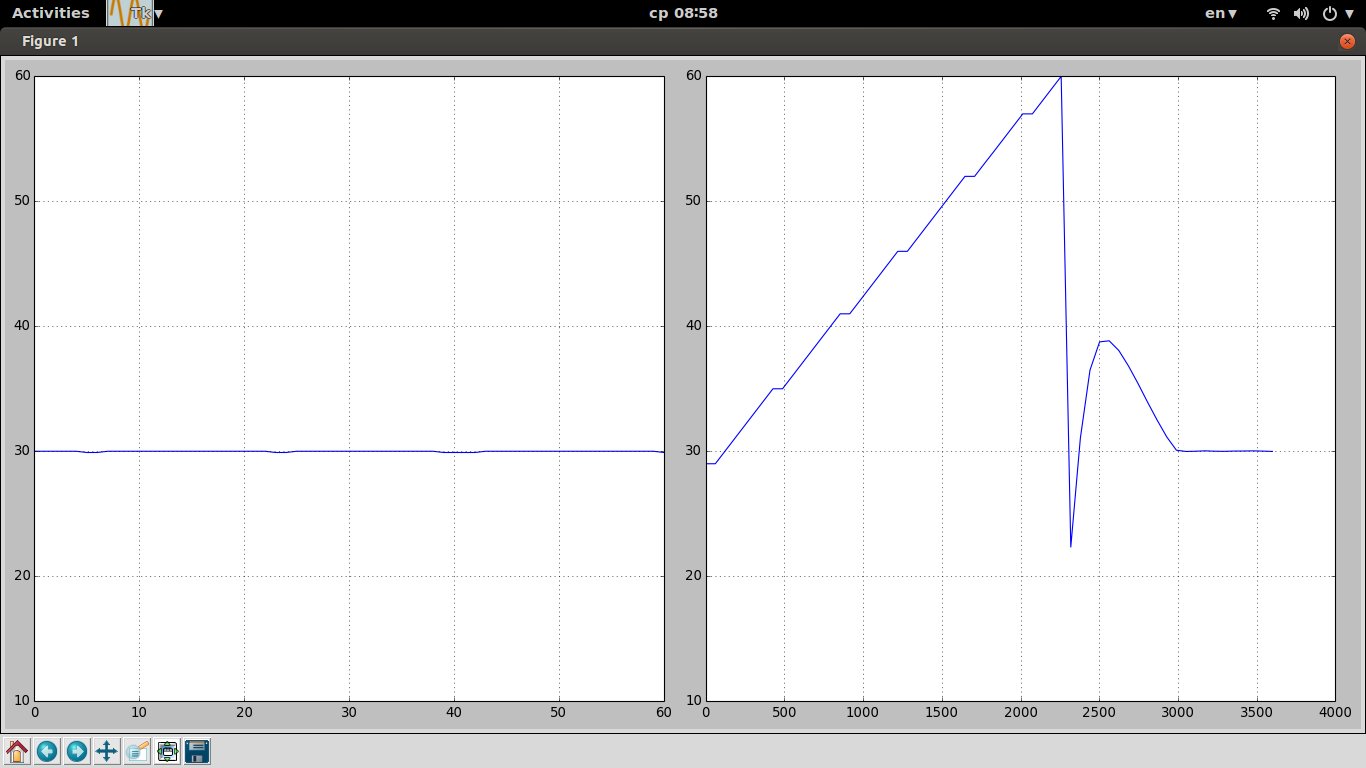
\includegraphics[width=0.8\textwidth]{../images/exp_gain100}~
\end{frame}

\begin{frame}
\frametitle{Astrom-Hagglund sustained oscillation mode}
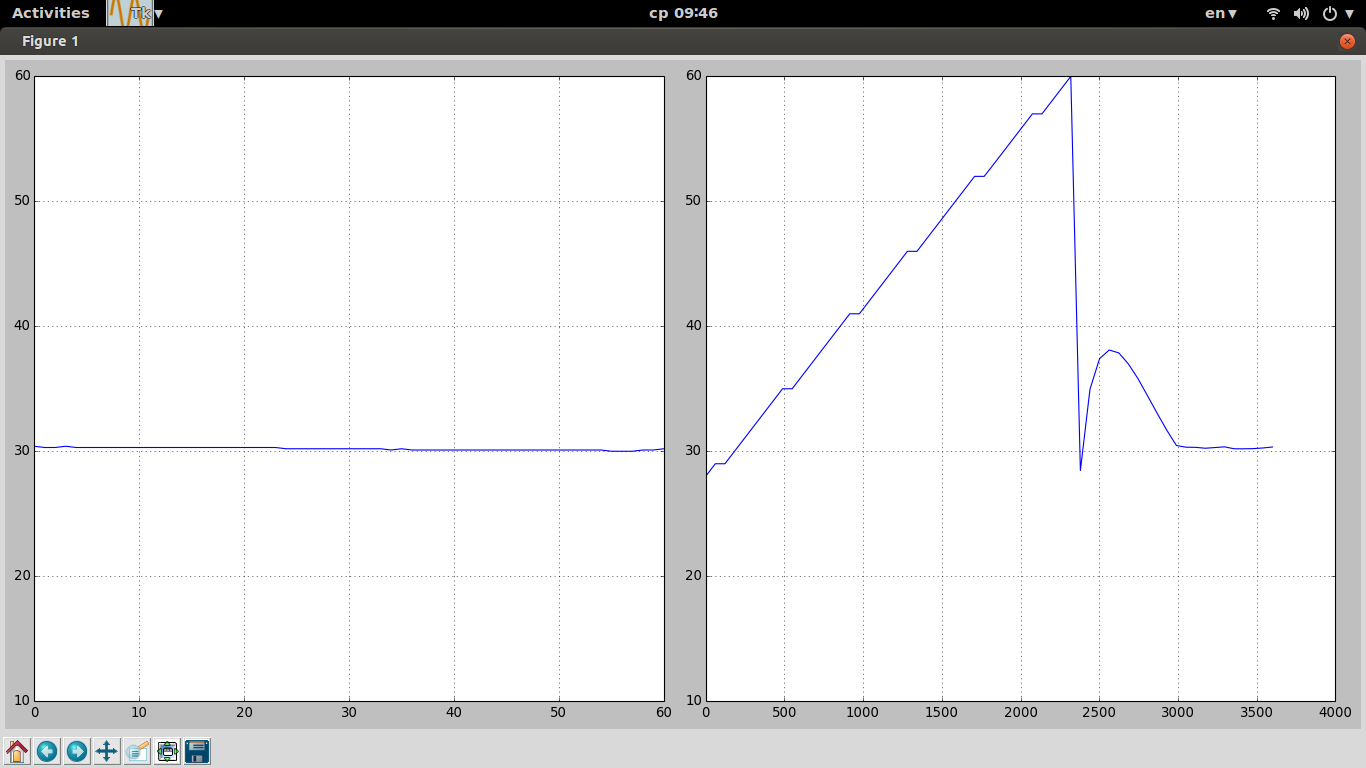
\includegraphics[width=0.8\textwidth]{../images/exp_relay}~
\end{frame}

\begin{frame}

\frametitle{Sampling frequency reduced}
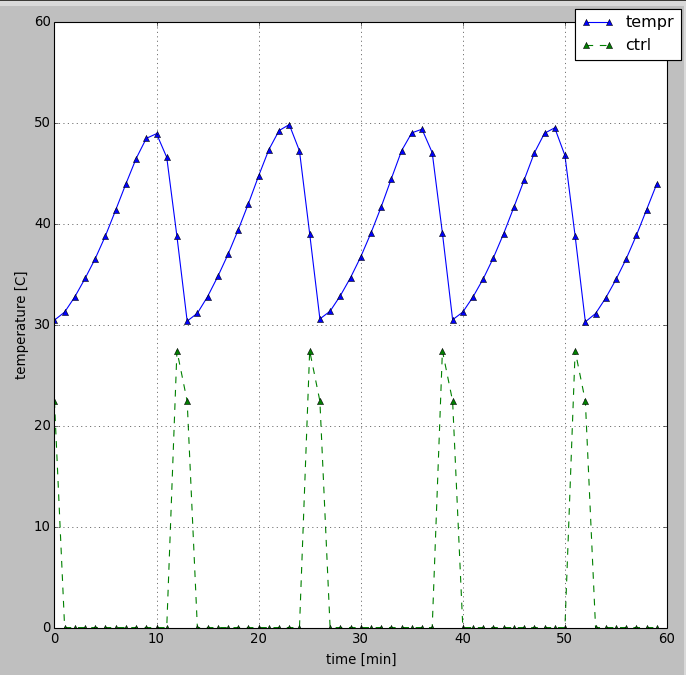
\includegraphics[width=0.8\textwidth]{../images/exp_relay_slow}~
\end{frame}

\begin{frame}
\frametitle{Thank you!}
Questions?
\end{frame}

\end{document}
